\begin{flushright} {\tiny {\color{gray} fdm\_basics1D.tex}} \end{flushright}
%~~~~~~~~~~~~~~~~~~~~~~~~~~~~~~~~~~~~~~~~~~~~~~~~~~~~~~~~~~~~~~~~~~~~~~~~~~~~~~~~~~~~~~~~~~~~~~~~~~

In what follows we suppose that we have a function $f(x)$, 
which is continuous and differentiable over the range of interest. 
Let us also assume that we know the value $f(x_0)$ and all the derivatives at $x = x_0$. 

%.......................................
\subsection{First order derivatives}

The forward Taylor-series expansion for $f(x_0 + h)$, away 
from the point $x_0$ by a small amount $h$ is given by
\begin{equation}
f(x_0+h)=f(x_0)+ 
h \frac{\partial f}{\partial x}(x_0)  + 
\frac{h^2}{2!} \frac{\partial^2 f}{\partial x^2}(x_0)  +
\dots  +
\frac{h^n}{n!} \frac{\partial^n f}{\partial x^n}(x_0)  
+ {\cal O}(h^{n+1})
\end{equation}
We can substract $f(x_0)$ to each side of the equation and divide by $h$:
\begin{equation}
\frac{1}{h} \left[f(x_0+h)-f(x_0)\right] = 
 \frac{\partial f}{\partial x}(x_0)  + 
\frac{h}{2!} \frac{\partial^2 f}{\partial x^2}(x_0)  + \dots 
\end{equation}
and we can then express the first derivative of $f$ as follows:
\begin{equation}
\frac{\partial f}{\partial x}(x_0) = \frac{f(x_0+h)-f(x_0)}{h} - 
\frac{h}{2!} \frac{\partial^2 f}{\partial x^2}(x_0)  \dots
\end{equation}
or, replacing the term in $h$ by ${\cal O}(h)$:
\begin{equation}
\boxed{
\frac{\partial f}{\partial x}(x_0) = \frac{f(x_0+h)-f(x_0)}{h} + {\cal O}(h)
}
\end{equation}
${\cal O}(h)$ indicates that the full solution would require additional terms of order $h$, $h^2$, 
and so on. ${\cal O}$ is called the {\color{olive}truncation error}: if the distance $h$ 
is made smaller and smaller, the (numerical approximation) error decreases $\propto$ $h$ in this case.

\index{general}{Truncation Error}

Let us assume that the 1D domain on which a given Ordinary Differential 
Equation (ODE) or Partial Differential Equation (PDE) is to be solved has been discretised
and let us zoom in on three consecutive points ($x_0=x_i$ here):

\begin{center}
\input{tikz/tikz_fdm1Da}
\end{center}

\noindent In the context of a discrete calculation on a set of discrete points $x_i$
we can compute the first order derivative of $f$ at point $x_i$ as an approximation:

\begin{equation}
\boxed{
\frac{\partial f}{\partial x}(x_i) = \frac{f_{i+1}-f_i}{h} + {\cal O}(h) 
}
\qquad
\qquad
\text{(forward difference)} 
\end{equation}
where functions $f_i = f (x_i)$ are evaluated at discretely spaced $x_i$ with $x_{i+1} = x_i + h$ 
(i.e. $h=x_{i+1}-x_i$), where the node spacing, or resolution, $h$ is assumed constant.
We also introduce the notation $f_i'=f'(x_i)=\frac{\partial f}{\partial x} (x_i)$. 


The {\bf forward FD derivative} as expressed above is called {\bf first order accurate},
and this means that very small $h$ is required for an accurate solution.
\index{general}{Forward FD Derivative}
\index{general}{Truncation Error}

%/-/-/-/-/-/-/-/-/-/-/-/-/-/-/-/-/-/-/-/
\begin{center}
\begin{minipage}[t]{0.77\textwidth}
\par\noindent\rule{\textwidth}{0.4pt}
{\color{blue}Example FDM-1:} Before we go any further with the theory, let us look at a very simple example. 
Let us consider the Stokes equations in the absence of fluid motion (i.e. $\vec\upnu=\vec 0$).
Then the strain rate tensor components are identically zero and the equation simply is 
\begin{equation}
-\vec\nabla p + \rho \vec{g} = \vec 0.
\end{equation}
where we assume that 1) density is constant in space for simplicity and 2)
the domain is infinite in the $x$-direction.
The gravity vector is $\vec{g}=-g \vec{e}_y$ so that the above equation 
becomes:
\begin{equation}
-\frac{dp}{dy} - \rho g = 0
\end{equation}
This is a first-order ODE. It needs to be supplemented by a single boundary condition, 
which in this case constrains the pressure to be zero at the surface, i.e. $p(y=L_y)=0$.

\begin{center}
\input{tikz/tikz_fdm1De}
\end{center}

We can write the discretised ODE at node 2 (since we know $p_3=0$):
\begin{equation}
\frac{dp}{dy}(x_2) \simeq \frac{p_3-p_2}{h} = -\rho g
\end{equation}
or, $p_2=\rho g h$. Having obtained $p_2$, we write the ODE at node 1:
\begin{equation}
\frac{dp}{dy}(x_1) \simeq \frac{p_2-p_1}{h} = -\rho g
\end{equation}
or, $p_1= \rho g h + p_2 = \rho g 2h$. And finally we obtain as expected
\begin{equation}
p_0 = \rho g \; 3h = \rho g L_y.
\end{equation}

\par\noindent\rule{\textwidth}{0.4pt}
\end{minipage}
\end{center}

\newpage
This brings us to our first exercise:

\begin{center}
\begin{minipage}[t]{0.77\textwidth}
\par\noindent\rule{\textwidth}{0.4pt}

\begin{center}
\includegraphics[width=0.8cm]{images/garftr} \\
{\color{orange}Exercise FDM-1}
\end{center}

We will now put the previous example into practice and write a 
python code which uses forward differences to compute the 1D pressure
field inside the crust.

\begin{verbatim}
import numpy as np
import matplotlib as mpl 
import matplotlib.pyplot as plt 
Ly=30e3
nny=10
g=9.81
rho=3000
#Compute , the distance between nodes
h=
#declare/fill the y array 
y=

#Set the pressure at the top to zero and work backwards to compute the pressure at the remaining nodes.

#Print the expected value at the bottom next to the computed value at y=0

plt.figure(figsize=(6,5)) #Size of figure in inches (or 'freedom units'), x,y
plt.title('Pressure Profile')
plt.plot(p,y,color='black')
plt.xlabel('Pressure (N/m2)')
plt.ylabel('Vertical Profile (m)')
plt.grid()
plt.savefig('PressureProfile.pdf')
\end{verbatim}

\par\noindent\rule{\textwidth}{0.4pt}
\end{minipage}
\end{center}
%/-/-/-/-/-/-/-/-/-/-/-/-/-/-/-/-/-/-/-/


\newpage

\noindent We can also expand the Taylor series backward (i.e. looking 'left' of $x_0$)
\begin{equation}
f(x_0-h)=f(x_0)-
h \frac{\partial f}{\partial x}(x_0)  + 
\frac{h^2}{2!} \frac{\partial^2 f}{\partial x^2}(x_0)  -
\dots 
\end{equation}
The {\bf backward FD derivative} then writes:
\begin{equation}
\boxed{
\frac{\partial f}{\partial x}(x_i) = \frac{f_{i}-f_{i-1}}{h} + {\cal O}(h) 
}
\qquad
\qquad
\text{(backward difference)} 
\end{equation}

\index{general}{Backward FD Derivative}



Alternatively, we can substract the backward formula from the forward one 
and divide by two; concretely, we start from 
\begin{equation}
f(x_0+h)=f(x_0)+ 
h \frac{\partial f}{\partial x}(x_0)  + 
\frac{h^2}{2!} \frac{\partial^2 f}{\partial x^2}(x_0)  + \dots  
\end{equation}
and substract the following from it
\begin{equation}
f(x_0-h)=f(x_0)-
h \frac{\partial f}{\partial x}(x_0)  + 
\frac{h^2}{2!} \frac{\partial^2 f}{\partial x^2}(x_0)  + \dots 
\end{equation}
to obtain:
\begin{equation}
f(x_0+h)-f(x_0-h) = 2h \frac{\partial f}{\partial x}(x_0)  +{\cal O}(h^3) 
\end{equation}
or, 
\[
\frac{\partial f}{\partial x}(x_0)  = \frac{ f(x_0+h)-f(x_0-h)}{2h} +{\cal O}(h^2) 
\]
We see that the resulting {\bf central difference} approximation is 
{\bf second order accurate}. In the discrete world one then write
\begin{equation}
\boxed{
\frac{\partial f}{\partial x}(x_i) 
= \frac{f_{i+1}-f_{i-1}}{2h} + {\cal O}(h^2)
}
\qquad
\qquad
\text{(central difference)} 
\end{equation}
Simply put, the denominator is $2h$ because it is the distance between point $x_{i-1}$ and $x_{i+1}$.


\begin{center}
\includegraphics[width=8cm]{images/fdm/fd1}\\
{\captionfont 
3 types of the finite difference method. Central gives the best approximation of the derivative.
Taken from Wikipedia\footnote{\url{https://en.wikipedia.org/wiki/Finite_difference}}
}
\end{center}

Can we do better than ${\cal O}(h^2)$? The answer is yes, and I list hereunder the 
formula:
\begin{equation}
\frac{\partial f}{\partial x}(x_i) 
= \frac{2 f_{i+1} + 3 f_i - 6 f_{i-1} + f_{i-2}}{6 h} + {\cal O}(h^3)
\qquad
\text{backward difference}
\end{equation}

\begin{equation}
\frac{\partial f}{\partial x}(x_i) 
= \frac{-  f_{i+2} +6 f_{i+1} - 3 f_{i} -2 f_{i-1}}{6 h} + {\cal O}(h^3)
\qquad
\text{forward difference}
\end{equation}

\begin{equation}
\frac{\partial f}{\partial x}(x_i) 
= \frac{-  f_{i+2} +8 f_{i+1} - 8 f_{i-1} + f_{i-2}}{12 h} + {\cal O}(h^4)
\qquad
\text{central difference}
\end{equation}
Looking at these formula it is obvious that the cost of forming the derivative 
is larger than before (more multiplications, additions, ...) which translates
to longer calculations and, in the case of implicit methods, much denser matrices. 


\begin{center}
\begin{minipage}[t]{0.77\textwidth}
\par\noindent\rule{\textwidth}{0.4pt}

\begin{center}
\includegraphics[width=0.8cm]{images/garftr} \\
{\color{orange}Exercise FDM-1 (bonus)}
\end{center}

Prove the formula above.

\par\noindent\rule{\textwidth}{0.4pt}
\end{minipage}
\end{center}
%/-/-/-/-/-/-/-/-/-/-/-/-/-/-/-/-/-/-/-/


%.......................................
\subsection{Second-order derivatives - simple case}

Many PDEs contain second order derivatives (typically diffusion equations or wave equations)
so we now turn to these and 
define $f_i''=f''(x_i) = \frac{d^2 f}{d x^2} (x_i)$. 

%______________________________
\paragraph{Second order derivative - forward} 
Let us define a function $g(x)$ such that $g=f'$. Then we have seen that the forward 
difference formula leads to write: 
\begin{equation}
g_i' = \frac{g_{i+1}-g_{i}}{h}
\end{equation}
On the one hand, we have $g_i'=g'(x_i)=f''(x_i)=f_i''$ and on the other hand
\begin{equation}
\frac{g_{i+1}-g_{i}}{h} = \frac{f_{i+1}'-f_{i}'}{h}
\end{equation}
We can then use the forward derivative formula for $f_{i+1}'$ and $f_{i}'$ and 
obtain the following second order derivatives of $f$:
\begin{equation}
f_{i}'' 
= \frac{f_{i+1}'-f_i'}{h} 
%+ {\cal O}(h^2)
= \frac{\frac{f_{i+2}-f_{i+1}}{h}-
\frac{f_{i+1}-f_i}{h}
}{h} 
%+ {\cal O}(h^2)
= \frac{f_{i+2}-2f_{i+1}+f_i}{h^2} 
%+ {\cal O}(h^2)
\end{equation}
which is the {\bf first order accurate}, {\bf forward difference} approximation for
second order derivatives at $x_{i}$.
In order to compute $f''(x_i)$ we need the value of $f$ at $x_i$ but also at two 
other locations right of this location.

%______________________________
\paragraph{Second order derivative - backward}
Likewise, we obtain the following formula when using the backward derivative twice:

\begin{equation}
f_{i}'' 
= \frac{f_{i}'-f_{i-1}'}{h} 
%+ {\cal O}(h^2)
= \frac{\frac{f_{i}-f_{i-1}}{h}- \frac{f_{i-1}-f_{i-2}}{h}  }{h} 
%+ {\cal O}(h^2)
= \frac{f_{i}-2f_{i-1}+f_{i-2}}{h^2} 
%+ {\cal O}(h^2)
\end{equation}
This time we  we need the value of $f$ at $x_i$ but also at two 
other locations left of this location.

%______________________________
\paragraph{Second order central} 
By adding the taylor expansions (with $+h$ and $-h$) 
a {\bf second order accurate}  approximation of the second derivative is obtained.
We start from 

\begin{eqnarray}
f(x_0+h)&=&f(x_0)+ 
h \frac{\partial f}{\partial x}(x_0)  + 
\frac{h^2}{2!} \frac{\partial^2 f}{\partial x^2}(x_0)  +
\frac{h^3}{3!} \frac{\partial^3 f}{\partial x^3}(x_0)  +
\dots  +
\frac{h^n}{n!} \frac{\partial^n f}{\partial x^n}(x_0)  
+ {\cal O}(h^{n+1}) 
\nn\\
f(x_0-h)&=&f(x_0) 
-h \frac{\partial f}{\partial x}(x_0)  + 
\frac{h^2}{2!} \frac{\partial^2 f}{\partial x^2}(x_0)  -
\frac{h^3}{3!} \frac{\partial^3 f}{\partial x^3}(x_0)  +
\dots  +
\frac{(-h)^n}{n!} \frac{\partial^n f}{\partial x^n}(x_0)  
+ {\cal O}(h^{n+1}) \nn
\end{eqnarray}
and we see that adding the first equation to the second yields
\begin{equation}
f(x_0+h) + f(x_0-h) =2 f(x_0)+ 
\underbrace{h \frac{\partial f}{\partial x}(x_0)   
-h \frac{\partial f}{\partial x}(x_0)}_{=0}  + 
2\frac{h^2}{2!} \frac{\partial^2 f}{\partial x^2}(x_0)  
+
\underbrace{
\frac{h^3}{3!} \frac{\partial^3 f}{\partial x^3}(x_0)  
-\frac{h^3}{3!} \frac{\partial^3 f}{\partial x^3}(x_0)  
}_{=0}
+ {\cal O}(h^{4})
\end{equation}
or, 
\begin{equation}
\frac{\partial^2 f}{\partial x^2}(x_0)  =
\frac{f(x_0+h) -2f(x_0) + f(x_0-h) }{h^2}
+ {\cal O}(h^2)
\end{equation}
which translates into
\begin{equation}
\boxed{
f_{i}''=\frac{f_{i+1}-2f_i+f_{i-1}}{h^2} + {\cal O}(h^2)
}
\qquad
\qquad
\text{(second order central difference)}
\label{eq:fpp1}
\end{equation}
Note that this formula requires one value left and one value right of the point 
under consideration. 

\noindent Can we do better than ${\cal O}(h^2)$? The answer is yes again:
\begin{equation}
f_i'' = \frac{-f_{i+2} + 16 f_{i+1} -30 f_i + 16 f_{i-1} - f_{i-2} }{12 h^2} + {\cal O}(h^4)
\label{eq:fpp2}
\end{equation}

Note that in some cases the fully forward or backward expressions 
need to be used on the boundary if the value of the function is not prescribed.

%------------------------------------------------------------------------
\subsection{Second-order derivatives - spatially varying coeffs \& mesh cell size}

Another way to arrive at the same expression is to write the expansion at $x_0 \pm h/2$, 
i.e. at the (convenient, yet nonexistent) half points $i\pm 1/2$:

\begin{center}
\input{tikz/tikz_fdm1Db}
\end{center}


%\begin{verbatim}
%     
%                              x_{i-1/2)           x_{i+1/2}
%               --------|----------+----------|---------+----------|-------------> x
%                     x_{i-1}                x_i                x_{i+1}
%
%\end{verbatim}

\begin{equation}
f_{i+1/2}'=\frac{f_{i+1}-f_i}{h}
\quad\quad
\quad\quad
f_{i-1/2}'=\frac{f_{i}-f_{i-1}}{h}
\end{equation}
\begin{equation}
f_i''=\frac{f_{i+1/2}'-f_{i-1/2}'}{h} = 
\frac{f_{i+1}-2f_i+f_{i-1}}{h^2} 
\end{equation}

Note that derivatives of the form (see heat transport equation in Section~\ref{ss:hte}) 
\begin{equation}
\frac{\partial }{\partial x} \left(  k  \frac{\partial f}{\partial x} \right)
\end{equation}
where $k$ is a function of space, should be formed as follows
\begin{equation}
\left. \frac{\partial }{\partial x} \left(  k  \frac{\partial f}{\partial x} \right) \right|_i
=
\frac{ k_{i+1/2} \frac{f_{i+1}-f_i}{h} - k_{i-1/2}\frac{f_i-f_{i-1}}{h}    }{h} + {\cal O}(h^2)
\label{eq:fdm_discterms}
\end{equation}
where $k_{i\pm 1/2}$ is evaluated between the points to maintain the second order accuracy.
One typically use an arithmetic averaging but harmonic averaging too \cite{gery19book}.

\begin{remark}
If the heat conductivity $k$ shows strong jumps from one grid point to another that are not aligned with
the grid-nodes, most second-order methods will show first order accuracy at best.
\end{remark}

Let us now consider the generic case where nodes are not equidistant and mesh spacing can also vary:
\begin{center}
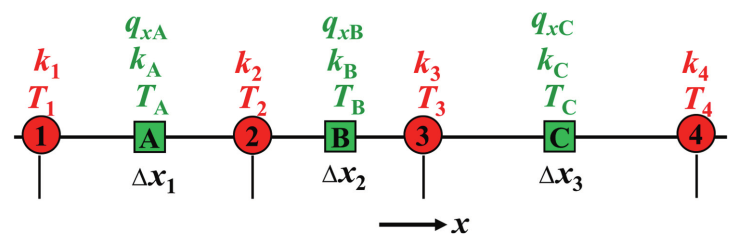
\includegraphics[width=10cm]{python_codes/fieldstone_180/gerya_stencil}\\
{\captionfont I need to redo the figure and replace $\Delta x_i$ by $h_i$.}
\end{center}
We denote by A,B,C the positions of the middle of each cell.

Following Section 10.2 of \textcite{gery19book}, we follow the
proposed {\it conservative} Finite Difference formulation of the flux terms
and we write the heat flux at nodes 2 and 3 as follows:
\begin{eqnarray}
\left.\frac{dq}{dx}\right|_2 &=& \frac{q_B-q_A}{(h_1+h_2)/2} \nn\\
\left.\frac{dq}{dx}\right|_3 &=& \frac{q_C-q_B}{(h_2+h_3)/2} \nn
\end{eqnarray}

We choose\footnote{Note that in the book Gerya presents 
another way of averaging the conductivity, i.e. a harmonic averaging.} 
\[
k_A = \frac{k_1+k_2}{2}
\qquad
k_B = \frac{k_2+k_3}{2}
\qquad
k_C = \frac{k_3+k_4}{2}
\]
so that we have for instance
\begin{eqnarray}
\left.\frac{dq}{dx}\right|_3
&=& \frac{q_C-q_B}{(h_2+h_3)/2} \nn\\
&=& \frac{-k_C \frac{T_4-T_3}{h_3} + k_B \frac{T_3-T_2}{h_2}  }{(h_2+h_3)/2} \nn\\
&=& \frac{- \frac{k_3+k_4}{2} \frac{T_4-T_3}{h_3} + \frac{k_2+k_3}{2} \frac{T_3-T_2}{h_2}  }{(h_2+h_3)/2} \nn\\
&=& -\frac{k_3+k_4}{h_3(h_2+h_3)} (T_4-T_3)+  \frac{k_2+k_3}{h_2(h_2+h_3)} (T_3-T_2)\nn
\end{eqnarray}
and finally
\[
\left.\frac{dq}{dx}\right|_3
=
-\frac{k_2+k_3}{h_2(h_2+h_3)} T_2
+ \left(
\frac{k_3+k_4}{h_3(h_2+h_3)} + \frac{k_2+k_3}{h_2(h_2+h_3)} 
\right) T_3
-\frac{k_3+k_4}{h_3(h_2+h_3)} T_4
\]
This leads in the end to the following stencil for the inside nodes:
\[
\frac{dq}{dx}|_i
= - \frac{k_{i-1}+k_i}{h_{i-1} (h_{i-1}+h_i)} T_{i-1}
+\left(
\frac{k_{i}+k_{i+1}}{h_{i} (h_{i-1}+h_i)} +
\frac{k_{i-1}+k_i}{h_{i-1} (h_{i-1}+h_i)}
\right) T_i
 - \frac{k_{i}+k_{i+1}}{h_{i} (h_{i-1}+h_i)} T_{i+1}
\]
Note that stencil does not lead to symmetric matrix, even for a diffusion equation!

Of course it is trivial to verify that if the node spacing is constant and the 
heat conductivity is also constant then the stencil above simply becomes 
\[
\frac{dq}{dx}|_i = -k \frac{T_{i-1}-2T_i+T_{i+1}}{h^2}
\] 
Likewise, we can derive the stencil for a varying heat conductivity
but constant mesh spacing:
\[
\frac{dq}{dx}|_i
= 
- \frac{k_{i-1}+k_i}{2h^2} T_{i-1}
+\left(
\frac{k_{i}+k_{i+1}}{2h^2} + \frac{k_{i-1}+k_i}{2h^2}
\right) T_i
 - \frac{k_{i}+k_{i+1}}{2h^2} T_{i+1}
=
- \frac{k_{i-1}+k_i}{2h^2} T_{i-1}
+\frac{k_{i-1}+ 2k_{i}+k_{i+1}}{2h^2} T_i
- \frac{k_{i}+k_{i+1}}{2h^2} T_{i+1}
\]
which is identical to Eq.~\eqref{eq:fdm_discterms}.






